\documentclass[a4paper,11pt]{article}%,twocolumn
%% packages


\usepackage{amsmath} % needed for command eqref
\usepackage{amssymb} % needed for math fonts
\usepackage[colorlinks=true,breaklinks]{hyperref} % needed for creating hyperlinks in the document, the option colorlinks=true gets rid of the awful boxes, breaklinks breaks lonkg links (list of figures), and ngerman sets everything for german as default hyperlinks language
\usepackage[hyphenbreaks]{breakurl} % ben�tigt f�r das Brechen von URLs in Literaturreferenzen, hyphenbreaks auch bei links, die �ber eine Seite gehen (mit hyphenation).
\usepackage{xcolor}
\definecolor{c1}{rgb}{0,0,1} % blue
\definecolor{c2}{rgb}{0,0.3,0.9} % light blue
\definecolor{c3}{rgb}{0.3,0,0.9} % red blue
\hypersetup{
    linkcolor={c1}, % internal links
    citecolor={c2}, % citations
    urlcolor={c3} % external links/urls
}
%\usepackage{cite} % needed for cite
\usepackage[square,authoryear]{natbib} % needed for cite and abbrvnat bibliography style
\usepackage[nottoc]{tocbibind} % needed for displaying bibliography and other in the table of contents
\usepackage{graphicx} % needed for \includegraphics 
\usepackage{longtable} % needed for long tables over pages
\usepackage{bigstrut} % needed for the command \bigstrut
\usepackage{enumerate} % needed for some options in enumerate
%\usepackage{todonotes} % needed for todos
\usepackage{makeidx} % needed for creating an index
\makeindex
\usepackage{gensymb}
\usepackage{url}
\usepackage{psfrag}
\usepackage{multirow}
\usepackage{subfigure}
\usepackage{epstopdf}

%% page settings

\usepackage[top=20mm, bottom=20mm,left=20mm,right=20mm]{geometry} % needed for page border settings
\parindent=0mm % for space of first line of new text block
\sloppy % for writing with hyphenless justification (tries to)
\hyphenation{} % use hyphenation of tolerance parametershttp://www.jr-x.de/publikationen/latex/tipps/zeilenumbruch.html
\hyphenpenalty=10000
\exhyphenpenalty=10000
\usepackage{fancyhdr} % needed for head and foot options
    \usepackage[breakable]{tcolorbox}
    \usepackage{xcolor} % Allow colors to be defined  
    \usepackage{textcomp} % defines textquotesingle
    \usepackage{upquote} % Upright quotes for verbatim code
    \usepackage{eurosym} % defines \euro
    \usepackage[mathletters]{ucs} % Extended unicode (utf-8) support
    \usepackage{fancyvrb} % verbatim replacement that allows latex
    \usepackage{grffile} % extends the file name processing of package graphics 
                         % to support a larger range
    \makeatletter % fix for old versions of grffile with XeLaTeX
    \@ifpackagelater{grffile}{2019/11/01}
    {
      % Do nothing on new versions
    }
    {
      \def\Gread@@xetex#1{%
        \IfFileExists{"\Gin@base".bb}%
        {\Gread@eps{\Gin@base.bb}}%
        {\Gread@@xetex@aux#1}%
      }
    }
    \makeatother
    \usepackage{titling}
    \usepackage{longtable} % longtable support required by pandoc >1.10
    \usepackage{booktabs}  % table support for pandoc > 1.12.2
    \usepackage[inline]{enumitem} % IRkernel/repr support (it uses the enumerate* environment)
    \usepackage[normalem]{ulem} % ulem is needed to support strikethroughs (\sout)
                                % normalem makes italics be italics, not underlines
    \usepackage{mathrsfs}
    

    % ANSI colors
    \definecolor{ansi-black}{HTML}{3E424D}
    \definecolor{ansi-black-intense}{HTML}{282C36}
    \definecolor{ansi-red}{HTML}{E75C58}
    \definecolor{ansi-red-intense}{HTML}{B22B31}
    \definecolor{ansi-green}{HTML}{00A250}
    \definecolor{ansi-green-intense}{HTML}{007427}
    \definecolor{ansi-yellow}{HTML}{DDB62B}
    \definecolor{ansi-yellow-intense}{HTML}{B27D12}
    \definecolor{ansi-blue}{HTML}{208FFB}
    \definecolor{ansi-blue-intense}{HTML}{0065CA}
    \definecolor{ansi-magenta}{HTML}{D160C4}
    \definecolor{ansi-magenta-intense}{HTML}{A03196}
    \definecolor{ansi-cyan}{HTML}{60C6C8}
    \definecolor{ansi-cyan-intense}{HTML}{258F8F}
    \definecolor{ansi-white}{HTML}{C5C1B4}
    \definecolor{ansi-white-intense}{HTML}{A1A6B2}
    \definecolor{ansi-default-inverse-fg}{HTML}{FFFFFF}
    \definecolor{ansi-default-inverse-bg}{HTML}{000000}

    % common color for the border for error outputs.
    \definecolor{outerrorbackground}{HTML}{FFDFDF}

    % commands and environments needed by pandoc snippets
    % extracted from the output of `pandoc -s`
    \providecommand{\tightlist}{%
      \setlength{\itemsep}{0pt}\setlength{\parskip}{0pt}}
    \DefineVerbatimEnvironment{Highlighting}{Verbatim}{commandchars=\\\{\}}
    %' for more characters per line
    \newenvironment{Shaded}{}{}
    \newcommand{\KeywordTok}[1]{\textcolor[rgb]{0.00,0.44,0.13}{\textbf{{#1}}}}
    \newcommand{\DataTypeTok}[1]{\textcolor[rgb]{0.56,0.13,0.00}{{#1}}}
    \newcommand{\DecValTok}[1]{\textcolor[rgb]{0.25,0.63,0.44}{{#1}}}
    \newcommand{\BaseNTok}[1]{\textcolor[rgb]{0.25,0.63,0.44}{{#1}}}
    \newcommand{\FloatTok}[1]{\textcolor[rgb]{0.25,0.63,0.44}{{#1}}}
    \newcommand{\CharTok}[1]{\textcolor[rgb]{0.25,0.44,0.63}{{#1}}}
    \newcommand{\StringTok}[1]{\textcolor[rgb]{0.25,0.44,0.63}{{#1}}}
    \newcommand{\CommentTok}[1]{\textcolor[rgb]{0.38,0.63,0.69}{\textit{{#1}}}}
    \newcommand{\OtherTok}[1]{\textcolor[rgb]{0.00,0.44,0.13}{{#1}}}
    \newcommand{\AlertTok}[1]{\textcolor[rgb]{1.00,0.00,0.00}{\textbf{{#1}}}}
    \newcommand{\FunctionTok}[1]{\textcolor[rgb]{0.02,0.16,0.49}{{#1}}}
    \newcommand{\RegionMarkerTok}[1]{{#1}}
    \newcommand{\ErrorTok}[1]{\textcolor[rgb]{1.00,0.00,0.00}{\textbf{{#1}}}}
    \newcommand{\NormalTok}[1]{{#1}}
    
    % Additional commands for more recent versions of Pandoc
    \newcommand{\ConstantTok}[1]{\textcolor[rgb]{0.53,0.00,0.00}{{#1}}}
    \newcommand{\SpecialCharTok}[1]{\textcolor[rgb]{0.25,0.44,0.63}{{#1}}}
    \newcommand{\VerbatimStringTok}[1]{\textcolor[rgb]{0.25,0.44,0.63}{{#1}}}
    \newcommand{\SpecialStringTok}[1]{\textcolor[rgb]{0.73,0.40,0.53}{{#1}}}
    \newcommand{\ImportTok}[1]{{#1}}
    \newcommand{\DocumentationTok}[1]{\textcolor[rgb]{0.73,0.13,0.13}{\textit{{#1}}}}
    \newcommand{\AnnotationTok}[1]{\textcolor[rgb]{0.38,0.63,0.69}{\textbf{\textit{{#1}}}}}
    \newcommand{\CommentVarTok}[1]{\textcolor[rgb]{0.38,0.63,0.69}{\textbf{\textit{{#1}}}}}
    \newcommand{\VariableTok}[1]{\textcolor[rgb]{0.10,0.09,0.49}{{#1}}}
    \newcommand{\ControlFlowTok}[1]{\textcolor[rgb]{0.00,0.44,0.13}{\textbf{{#1}}}}
    \newcommand{\OperatorTok}[1]{\textcolor[rgb]{0.40,0.40,0.40}{{#1}}}
    \newcommand{\BuiltInTok}[1]{{#1}}
    \newcommand{\ExtensionTok}[1]{{#1}}
    \newcommand{\PreprocessorTok}[1]{\textcolor[rgb]{0.74,0.48,0.00}{{#1}}}
    \newcommand{\AttributeTok}[1]{\textcolor[rgb]{0.49,0.56,0.16}{{#1}}}
    \newcommand{\InformationTok}[1]{\textcolor[rgb]{0.38,0.63,0.69}{\textbf{\textit{{#1}}}}}
    \newcommand{\WarningTok}[1]{\textcolor[rgb]{0.38,0.63,0.69}{\textbf{\textit{{#1}}}}}
    
    
    % Define a nice break command that doesn't care if a line doesn't already
    % exist.
    \def\br{\hspace*{\fill} \\* }

% Pygments definitions
\makeatletter
\def\PY@reset{\let\PY@it=\relax \let\PY@bf=\relax%
    \let\PY@ul=\relax \let\PY@tc=\relax%
    \let\PY@bc=\relax \let\PY@ff=\relax}
\def\PY@tok#1{\csname PY@tok@#1\endcsname}
\def\PY@toks#1+{\ifx\relax#1\empty\else%
    \PY@tok{#1}\expandafter\PY@toks\fi}
\def\PY@do#1{\PY@bc{\PY@tc{\PY@ul{%
    \PY@it{\PY@bf{\PY@ff{#1}}}}}}}
\def\PY#1#2{\PY@reset\PY@toks#1+\relax+\PY@do{#2}}

\expandafter\def\csname PY@tok@w\endcsname{\def\PY@tc##1{\textcolor[rgb]{0.73,0.73,0.73}{##1}}}
\expandafter\def\csname PY@tok@c\endcsname{\let\PY@it=\textit\def\PY@tc##1{\textcolor[rgb]{0.25,0.50,0.50}{##1}}}
\expandafter\def\csname PY@tok@cp\endcsname{\def\PY@tc##1{\textcolor[rgb]{0.74,0.48,0.00}{##1}}}
\expandafter\def\csname PY@tok@k\endcsname{\let\PY@bf=\textbf\def\PY@tc##1{\textcolor[rgb]{0.00,0.50,0.00}{##1}}}
\expandafter\def\csname PY@tok@kp\endcsname{\def\PY@tc##1{\textcolor[rgb]{0.00,0.50,0.00}{##1}}}
\expandafter\def\csname PY@tok@kt\endcsname{\def\PY@tc##1{\textcolor[rgb]{0.69,0.00,0.25}{##1}}}
\expandafter\def\csname PY@tok@o\endcsname{\def\PY@tc##1{\textcolor[rgb]{0.40,0.40,0.40}{##1}}}
\expandafter\def\csname PY@tok@ow\endcsname{\let\PY@bf=\textbf\def\PY@tc##1{\textcolor[rgb]{0.67,0.13,1.00}{##1}}}
\expandafter\def\csname PY@tok@nb\endcsname{\def\PY@tc##1{\textcolor[rgb]{0.00,0.50,0.00}{##1}}}
\expandafter\def\csname PY@tok@nf\endcsname{\def\PY@tc##1{\textcolor[rgb]{0.00,0.00,1.00}{##1}}}
\expandafter\def\csname PY@tok@nc\endcsname{\let\PY@bf=\textbf\def\PY@tc##1{\textcolor[rgb]{0.00,0.00,1.00}{##1}}}
\expandafter\def\csname PY@tok@nn\endcsname{\let\PY@bf=\textbf\def\PY@tc##1{\textcolor[rgb]{0.00,0.00,1.00}{##1}}}
\expandafter\def\csname PY@tok@ne\endcsname{\let\PY@bf=\textbf\def\PY@tc##1{\textcolor[rgb]{0.82,0.25,0.23}{##1}}}
\expandafter\def\csname PY@tok@nv\endcsname{\def\PY@tc##1{\textcolor[rgb]{0.10,0.09,0.49}{##1}}}
\expandafter\def\csname PY@tok@no\endcsname{\def\PY@tc##1{\textcolor[rgb]{0.53,0.00,0.00}{##1}}}
\expandafter\def\csname PY@tok@nl\endcsname{\def\PY@tc##1{\textcolor[rgb]{0.63,0.63,0.00}{##1}}}
\expandafter\def\csname PY@tok@ni\endcsname{\let\PY@bf=\textbf\def\PY@tc##1{\textcolor[rgb]{0.60,0.60,0.60}{##1}}}
\expandafter\def\csname PY@tok@na\endcsname{\def\PY@tc##1{\textcolor[rgb]{0.49,0.56,0.16}{##1}}}
\expandafter\def\csname PY@tok@nt\endcsname{\let\PY@bf=\textbf\def\PY@tc##1{\textcolor[rgb]{0.00,0.50,0.00}{##1}}}
\expandafter\def\csname PY@tok@nd\endcsname{\def\PY@tc##1{\textcolor[rgb]{0.67,0.13,1.00}{##1}}}
\expandafter\def\csname PY@tok@s\endcsname{\def\PY@tc##1{\textcolor[rgb]{0.73,0.13,0.13}{##1}}}
\expandafter\def\csname PY@tok@sd\endcsname{\let\PY@it=\textit\def\PY@tc##1{\textcolor[rgb]{0.73,0.13,0.13}{##1}}}
\expandafter\def\csname PY@tok@si\endcsname{\let\PY@bf=\textbf\def\PY@tc##1{\textcolor[rgb]{0.73,0.40,0.53}{##1}}}
\expandafter\def\csname PY@tok@se\endcsname{\let\PY@bf=\textbf\def\PY@tc##1{\textcolor[rgb]{0.73,0.40,0.13}{##1}}}
\expandafter\def\csname PY@tok@sr\endcsname{\def\PY@tc##1{\textcolor[rgb]{0.73,0.40,0.53}{##1}}}
\expandafter\def\csname PY@tok@ss\endcsname{\def\PY@tc##1{\textcolor[rgb]{0.10,0.09,0.49}{##1}}}
\expandafter\def\csname PY@tok@sx\endcsname{\def\PY@tc##1{\textcolor[rgb]{0.00,0.50,0.00}{##1}}}
\expandafter\def\csname PY@tok@m\endcsname{\def\PY@tc##1{\textcolor[rgb]{0.40,0.40,0.40}{##1}}}
\expandafter\def\csname PY@tok@gh\endcsname{\let\PY@bf=\textbf\def\PY@tc##1{\textcolor[rgb]{0.00,0.00,0.50}{##1}}}
\expandafter\def\csname PY@tok@gu\endcsname{\let\PY@bf=\textbf\def\PY@tc##1{\textcolor[rgb]{0.50,0.00,0.50}{##1}}}
\expandafter\def\csname PY@tok@gd\endcsname{\def\PY@tc##1{\textcolor[rgb]{0.63,0.00,0.00}{##1}}}
\expandafter\def\csname PY@tok@gi\endcsname{\def\PY@tc##1{\textcolor[rgb]{0.00,0.63,0.00}{##1}}}
\expandafter\def\csname PY@tok@gr\endcsname{\def\PY@tc##1{\textcolor[rgb]{1.00,0.00,0.00}{##1}}}
\expandafter\def\csname PY@tok@ge\endcsname{\let\PY@it=\textit}
\expandafter\def\csname PY@tok@gs\endcsname{\let\PY@bf=\textbf}
\expandafter\def\csname PY@tok@gp\endcsname{\let\PY@bf=\textbf\def\PY@tc##1{\textcolor[rgb]{0.00,0.00,0.50}{##1}}}
\expandafter\def\csname PY@tok@go\endcsname{\def\PY@tc##1{\textcolor[rgb]{0.53,0.53,0.53}{##1}}}
\expandafter\def\csname PY@tok@gt\endcsname{\def\PY@tc##1{\textcolor[rgb]{0.00,0.27,0.87}{##1}}}
\expandafter\def\csname PY@tok@err\endcsname{\def\PY@bc##1{\setlength{\fboxsep}{0pt}\fcolorbox[rgb]{1.00,0.00,0.00}{1,1,1}{\strut ##1}}}
\expandafter\def\csname PY@tok@kc\endcsname{\let\PY@bf=\textbf\def\PY@tc##1{\textcolor[rgb]{0.00,0.50,0.00}{##1}}}
\expandafter\def\csname PY@tok@kd\endcsname{\let\PY@bf=\textbf\def\PY@tc##1{\textcolor[rgb]{0.00,0.50,0.00}{##1}}}
\expandafter\def\csname PY@tok@kn\endcsname{\let\PY@bf=\textbf\def\PY@tc##1{\textcolor[rgb]{0.00,0.50,0.00}{##1}}}
\expandafter\def\csname PY@tok@kr\endcsname{\let\PY@bf=\textbf\def\PY@tc##1{\textcolor[rgb]{0.00,0.50,0.00}{##1}}}
\expandafter\def\csname PY@tok@bp\endcsname{\def\PY@tc##1{\textcolor[rgb]{0.00,0.50,0.00}{##1}}}
\expandafter\def\csname PY@tok@fm\endcsname{\def\PY@tc##1{\textcolor[rgb]{0.00,0.00,1.00}{##1}}}
\expandafter\def\csname PY@tok@vc\endcsname{\def\PY@tc##1{\textcolor[rgb]{0.10,0.09,0.49}{##1}}}
\expandafter\def\csname PY@tok@vg\endcsname{\def\PY@tc##1{\textcolor[rgb]{0.10,0.09,0.49}{##1}}}
\expandafter\def\csname PY@tok@vi\endcsname{\def\PY@tc##1{\textcolor[rgb]{0.10,0.09,0.49}{##1}}}
\expandafter\def\csname PY@tok@vm\endcsname{\def\PY@tc##1{\textcolor[rgb]{0.10,0.09,0.49}{##1}}}
\expandafter\def\csname PY@tok@sa\endcsname{\def\PY@tc##1{\textcolor[rgb]{0.73,0.13,0.13}{##1}}}
\expandafter\def\csname PY@tok@sb\endcsname{\def\PY@tc##1{\textcolor[rgb]{0.73,0.13,0.13}{##1}}}
\expandafter\def\csname PY@tok@sc\endcsname{\def\PY@tc##1{\textcolor[rgb]{0.73,0.13,0.13}{##1}}}
\expandafter\def\csname PY@tok@dl\endcsname{\def\PY@tc##1{\textcolor[rgb]{0.73,0.13,0.13}{##1}}}
\expandafter\def\csname PY@tok@s2\endcsname{\def\PY@tc##1{\textcolor[rgb]{0.73,0.13,0.13}{##1}}}
\expandafter\def\csname PY@tok@sh\endcsname{\def\PY@tc##1{\textcolor[rgb]{0.73,0.13,0.13}{##1}}}
\expandafter\def\csname PY@tok@s1\endcsname{\def\PY@tc##1{\textcolor[rgb]{0.73,0.13,0.13}{##1}}}
\expandafter\def\csname PY@tok@mb\endcsname{\def\PY@tc##1{\textcolor[rgb]{0.40,0.40,0.40}{##1}}}
\expandafter\def\csname PY@tok@mf\endcsname{\def\PY@tc##1{\textcolor[rgb]{0.40,0.40,0.40}{##1}}}
\expandafter\def\csname PY@tok@mh\endcsname{\def\PY@tc##1{\textcolor[rgb]{0.40,0.40,0.40}{##1}}}
\expandafter\def\csname PY@tok@mi\endcsname{\def\PY@tc##1{\textcolor[rgb]{0.40,0.40,0.40}{##1}}}
\expandafter\def\csname PY@tok@il\endcsname{\def\PY@tc##1{\textcolor[rgb]{0.40,0.40,0.40}{##1}}}
\expandafter\def\csname PY@tok@mo\endcsname{\def\PY@tc##1{\textcolor[rgb]{0.40,0.40,0.40}{##1}}}
\expandafter\def\csname PY@tok@ch\endcsname{\let\PY@it=\textit\def\PY@tc##1{\textcolor[rgb]{0.25,0.50,0.50}{##1}}}
\expandafter\def\csname PY@tok@cm\endcsname{\let\PY@it=\textit\def\PY@tc##1{\textcolor[rgb]{0.25,0.50,0.50}{##1}}}
\expandafter\def\csname PY@tok@cpf\endcsname{\let\PY@it=\textit\def\PY@tc##1{\textcolor[rgb]{0.25,0.50,0.50}{##1}}}
\expandafter\def\csname PY@tok@c1\endcsname{\let\PY@it=\textit\def\PY@tc##1{\textcolor[rgb]{0.25,0.50,0.50}{##1}}}
\expandafter\def\csname PY@tok@cs\endcsname{\let\PY@it=\textit\def\PY@tc##1{\textcolor[rgb]{0.25,0.50,0.50}{##1}}}

\def\PYZbs{\char`\\}
\def\PYZus{\char`\_}
\def\PYZob{\char`\{}
\def\PYZcb{\char`\}}
\def\PYZca{\char`\^}
\def\PYZam{\char`\&}
\def\PYZlt{\char`\<}
\def\PYZgt{\char`\>}
\def\PYZsh{\char`\#}
\def\PYZpc{\char`\%}
\def\PYZdl{\char`\$}
\def\PYZhy{\char`\-}
\def\PYZsq{\char`\'}
\def\PYZdq{\char`\"}
\def\PYZti{\char`\~}
% for compatibility with earlier versions
\def\PYZat{@}
\def\PYZlb{[}
\def\PYZrb{]}
\makeatother


    % For linebreaks inside Verbatim environment from package fancyvrb. 
    \makeatletter
        \newbox\Wrappedcontinuationbox 
        \newbox\Wrappedvisiblespacebox 
        \newcommand*\Wrappedvisiblespace {\textcolor{red}{\textvisiblespace}} 
        \newcommand*\Wrappedcontinuationsymbol {\textcolor{red}{\llap{\tiny$\m@th\hookrightarrow$}}} 
        \newcommand*\Wrappedcontinuationindent {3ex } 
        \newcommand*\Wrappedafterbreak {\kern\Wrappedcontinuationindent\copy\Wrappedcontinuationbox} 
        % Take advantage of the already applied Pygments mark-up to insert 
        % potential linebreaks for TeX processing. 
        %        {, <, #, %, $, ' and ": go to next line. 
        %        _, }, ^, &, >, - and ~: stay at end of broken line. 
        % Use of \textquotesingle for straight quote. 
        \newcommand*\Wrappedbreaksatspecials {% 
            \def\PYGZus{\discretionary{\char`\_}{\Wrappedafterbreak}{\char`\_}}% 
            \def\PYGZob{\discretionary{}{\Wrappedafterbreak\char`\{}{\char`\{}}% 
            \def\PYGZcb{\discretionary{\char`\}}{\Wrappedafterbreak}{\char`\}}}% 
            \def\PYGZca{\discretionary{\char`\^}{\Wrappedafterbreak}{\char`\^}}% 
            \def\PYGZam{\discretionary{\char`\&}{\Wrappedafterbreak}{\char`\&}}% 
            \def\PYGZlt{\discretionary{}{\Wrappedafterbreak\char`\<}{\char`\<}}% 
            \def\PYGZgt{\discretionary{\char`\>}{\Wrappedafterbreak}{\char`\>}}% 
            \def\PYGZsh{\discretionary{}{\Wrappedafterbreak\char`\#}{\char`\#}}% 
            \def\PYGZpc{\discretionary{}{\Wrappedafterbreak\char`\%}{\char`\%}}% 
            \def\PYGZdl{\discretionary{}{\Wrappedafterbreak\char`\$}{\char`\$}}% 
            \def\PYGZhy{\discretionary{\char`\-}{\Wrappedafterbreak}{\char`\-}}% 
            \def\PYGZsq{\discretionary{}{\Wrappedafterbreak\textquotesingle}{\textquotesingle}}% 
            \def\PYGZdq{\discretionary{}{\Wrappedafterbreak\char`\"}{\char`\"}}% 
            \def\PYGZti{\discretionary{\char`\~}{\Wrappedafterbreak}{\char`\~}}% 
        } 
        % Some characters . , ; ? ! / are not pygmentized. 
        % This macro makes them "active" and they will insert potential linebreaks 
        \newcommand*\Wrappedbreaksatpunct {% 
            \lccode`\~`\.\lowercase{\def~}{\discretionary{\hbox{\char`\.}}{\Wrappedafterbreak}{\hbox{\char`\.}}}% 
            \lccode`\~`\,\lowercase{\def~}{\discretionary{\hbox{\char`\,}}{\Wrappedafterbreak}{\hbox{\char`\,}}}% 
            \lccode`\~`\;\lowercase{\def~}{\discretionary{\hbox{\char`\;}}{\Wrappedafterbreak}{\hbox{\char`\;}}}% 
            \lccode`\~`\:\lowercase{\def~}{\discretionary{\hbox{\char`\:}}{\Wrappedafterbreak}{\hbox{\char`\:}}}% 
            \lccode`\~`\?\lowercase{\def~}{\discretionary{\hbox{\char`\?}}{\Wrappedafterbreak}{\hbox{\char`\?}}}% 
            \lccode`\~`\!\lowercase{\def~}{\discretionary{\hbox{\char`\!}}{\Wrappedafterbreak}{\hbox{\char`\!}}}% 
            \lccode`\~`\/\lowercase{\def~}{\discretionary{\hbox{\char`\/}}{\Wrappedafterbreak}{\hbox{\char`\/}}}% 
            \catcode`\.\active
            \catcode`\,\active 
            \catcode`\;\active
            \catcode`\:\active
            \catcode`\?\active
            \catcode`\!\active
            \catcode`\/\active 
            \lccode`\~`\~ 	
        }
    \makeatother

    \let\OriginalVerbatim=\Verbatim
    \makeatletter
    \renewcommand{\Verbatim}[1][1]{%
        %\parskip\z@skip
        \sbox\Wrappedcontinuationbox {\Wrappedcontinuationsymbol}%
        \sbox\Wrappedvisiblespacebox {\FV@SetupFont\Wrappedvisiblespace}%
        \def\FancyVerbFormatLine ##1{\hsize\linewidth
            \vtop{\raggedright\hyphenpenalty\z@\exhyphenpenalty\z@
                \doublehyphendemerits\z@\finalhyphendemerits\z@
                \strut ##1\strut}%
        }%
        % If the linebreak is at a space, the latter will be displayed as visible
        % space at end of first line, and a continuation symbol starts next line.
        % Stretch/shrink are however usually zero for typewriter font.
        \def\FV@Space {%
            \nobreak\hskip\z@ plus\fontdimen3\font minus\fontdimen4\font
            \discretionary{\copy\Wrappedvisiblespacebox}{\Wrappedafterbreak}
            {\kern\fontdimen2\font}%
        }%
        
        % Allow breaks at special characters using \PYG... macros.
        \Wrappedbreaksatspecials
        % Breaks at punctuation characters . , ; ? ! and / need catcode=\active 	
        \OriginalVerbatim[#1,codes*=\Wrappedbreaksatpunct]%
    }
    \makeatother

    % Exact colors from NB
    \definecolor{incolor}{HTML}{303F9F}
    \definecolor{outcolor}{HTML}{D84315}
    \definecolor{cellborder}{HTML}{CFCFCF}
    \definecolor{cellbackground}{HTML}{F7F7F7}
    
    % prompt
    \makeatletter
    \newcommand{\boxspacing}{\kern\kvtcb@left@rule\kern\kvtcb@boxsep}
    \makeatother
    \newcommand{\prompt}[4]{
        {\ttfamily\llap{{\color{#2}[#3]:\hspace{3pt}#4}}\vspace{-\baselineskip}}
    }
    



\usepackage{fontawesome}
\usepackage{subfigure}

\begin{document}
    
	\begin{center}
	{\large \textbf{Assignment 3: EN4553 (Machine Vision)}}\\
	Thalagala B.P.\hspace{0.5cm} 180631J\\
	Submitted on \today
	
\end{center}
\hrule

%    \begin{tcolorbox}[breakable, size=fbox, boxrule=1pt, pad at break*=1mm,colback=cellbackground, colframe=cellborder]
%\prompt{In}{incolor}{1}{\boxspacing}
%\begin{Verbatim}[commandchars=\\\{\}]
%\PY{c+c1}{\PYZsh{} import required libraries}
%\PY{k+kn}{import} \PY{n+nn}{numpy} \PY{k}{as} \PY{n+nn}{np}
%\PY{k+kn}{import} \PY{n+nn}{matplotlib}\PY{n+nn}{.}\PY{n+nn}{pyplot} \PY{k}{as} \PY{n+nn}{plt}
%
%\PY{k+kn}{from} \PY{n+nn}{pathlib} \PY{k+kn}{import} \PY{n}{Path}
%\PY{k+kn}{from} \PY{n+nn}{typing} \PY{k+kn}{import} \PY{n}{Tuple}
%\PY{k+kn}{from} \PY{n+nn}{sklearn}\PY{n+nn}{.}\PY{n+nn}{linear\PYZus{}model} \PY{k+kn}{import} \PY{n}{LinearRegression}
%\PY{k+kn}{from} \PY{n+nn}{sklearn}\PY{n+nn}{.}\PY{n+nn}{metrics} \PY{k+kn}{import} \PY{n}{mean\PYZus{}squared\PYZus{}error}
%\end{Verbatim}
%\end{tcolorbox}

%    \begin{tcolorbox}[breakable, size=fbox, boxrule=1pt, pad at break*=1mm,colback=cellbackground, colframe=cellborder]
%\prompt{In}{incolor}{2}{\boxspacing}
%\begin{Verbatim}[commandchars=\\\{\}]
%\PY{c+c1}{\PYZsh{} setting parameters for pretty figures}
%\PY{n}{plt}\PY{o}{.}\PY{n}{rc}\PY{p}{(}\PY{l+s+s1}{\PYZsq{}}\PY{l+s+s1}{font}\PY{l+s+s1}{\PYZsq{}}\PY{p}{,} \PY{n}{size}\PY{o}{=}\PY{l+m+mi}{14}\PY{p}{)}
%\PY{n}{plt}\PY{o}{.}\PY{n}{rc}\PY{p}{(}\PY{l+s+s1}{\PYZsq{}}\PY{l+s+s1}{axes}\PY{l+s+s1}{\PYZsq{}}\PY{p}{,} \PY{n}{labelsize}\PY{o}{=}\PY{l+m+mi}{14}\PY{p}{,} \PY{n}{titlesize}\PY{o}{=}\PY{l+m+mi}{14}\PY{p}{)}
%\PY{n}{plt}\PY{o}{.}\PY{n}{rc}\PY{p}{(}\PY{l+s+s1}{\PYZsq{}}\PY{l+s+s1}{legend}\PY{l+s+s1}{\PYZsq{}}\PY{p}{,} \PY{n}{fontsize}\PY{o}{=}\PY{l+m+mi}{14}\PY{p}{)}
%\PY{n}{plt}\PY{o}{.}\PY{n}{rc}\PY{p}{(}\PY{l+s+s1}{\PYZsq{}}\PY{l+s+s1}{xtick}\PY{l+s+s1}{\PYZsq{}}\PY{p}{,} \PY{n}{labelsize}\PY{o}{=}\PY{l+m+mi}{10}\PY{p}{)}
%\PY{n}{plt}\PY{o}{.}\PY{n}{rc}\PY{p}{(}\PY{l+s+s1}{\PYZsq{}}\PY{l+s+s1}{ytick}\PY{l+s+s1}{\PYZsq{}}\PY{p}{,} \PY{n}{labelsize}\PY{o}{=}\PY{l+m+mi}{10}\PY{p}{)}
%
%\PY{c+c1}{\PYZsh{} fucntion to save figures}
%\PY{n}{IMAGES\PYZus{}PATH} \PY{o}{=} \PY{n}{Path}\PY{p}{(}\PY{p}{)} \PY{o}{/} \PY{l+s+s2}{\PYZdq{}}\PY{l+s+s2}{images}\PY{l+s+s2}{\PYZdq{}}
%\PY{n}{IMAGES\PYZus{}PATH}\PY{o}{.}\PY{n}{mkdir}\PY{p}{(}\PY{n}{parents}\PY{o}{=}\PY{k+kc}{True}\PY{p}{,} \PY{n}{exist\PYZus{}ok}\PY{o}{=}\PY{k+kc}{True}\PY{p}{)}
%
%\PY{k}{def} \PY{n+nf}{save\PYZus{}fig}\PY{p}{(}\PY{n}{fig\PYZus{}id}\PY{p}{,} \PY{n}{tight\PYZus{}layout}\PY{o}{=}\PY{k+kc}{True}\PY{p}{,} \PY{n}{fig\PYZus{}extension}\PY{o}{=}\PY{l+s+s2}{\PYZdq{}}\PY{l+s+s2}{png}\PY{l+s+s2}{\PYZdq{}}\PY{p}{,} \PY{n}{resolution}\PY{o}{=}\PY{l+m+mi}{300}\PY{p}{)}\PY{p}{:}
%    \PY{n}{path} \PY{o}{=} \PY{n}{IMAGES\PYZus{}PATH} \PY{o}{/} \PY{l+s+sa}{f}\PY{l+s+s2}{\PYZdq{}}\PY{l+s+si}{\PYZob{}}\PY{n}{fig\PYZus{}id}\PY{l+s+si}{\PYZcb{}}\PY{l+s+s2}{.}\PY{l+s+si}{\PYZob{}}\PY{n}{fig\PYZus{}extension}\PY{l+s+si}{\PYZcb{}}\PY{l+s+s2}{\PYZdq{}}
%    \PY{k}{if} \PY{n}{tight\PYZus{}layout}\PY{p}{:}
%        \PY{n}{plt}\PY{o}{.}\PY{n}{tight\PYZus{}layout}\PY{p}{(}\PY{p}{)}
%    \PY{n}{plt}\PY{o}{.}\PY{n}{savefig}\PY{p}{(}\PY{n}{path}\PY{p}{,} \PY{n+nb}{format}\PY{o}{=}\PY{n}{fig\PYZus{}extension}\PY{p}{,} \PY{n}{dpi}\PY{o}{=}\PY{n}{resolution}\PY{p}{)}
%\end{Verbatim}
%\end{tcolorbox}

    \hypertarget{a}{%
\section{(a)}\label{a}}

(5 points) Complete the following Python function to read the dataset as
a set of arrays. (Hint: you may use the \texttt{np.loadtxt()} function.)

    \begin{tcolorbox}[breakable, size=fbox, boxrule=1pt, pad at break*=1mm,colback=cellbackground, colframe=cellborder]
\prompt{In}{incolor}{3}{\boxspacing}
\begin{Verbatim}[commandchars=\\\{\}]
\PY{k}{def} \PY{n+nf}{load\PYZus{}dataset}\PY{p}{(} \PY{n}{src\PYZus{}dir}\PY{p}{:} \PY{n+nb}{str} \PY{p}{)} \PY{o}{\PYZhy{}}\PY{o}{\PYZgt{}} \PY{n}{Tuple}\PY{p}{[}\PY{n}{np}\PY{o}{.}\PY{n}{ndarray}\PY{p}{,} \PY{n}{np}\PY{o}{.}\PY{n}{ndarray}\PY{p}{,} \PY{n}{np}\PY{o}{.}\PY{n}{ndarray}\PY{p}{,} \PY{n}{np}\PY{o}{.}\PY{n}{ndarray}\PY{p}{,} \PY{n}{np}\PY{o}{.}\PY{n}{ndarray}\PY{p}{]}\PY{p}{:}
    \PY{l+s+sd}{\PYZdq{}\PYZdq{}\PYZdq{}Load the dataset as a set of numpy arrays.}
\PY{l+s+sd}{    Args:}
\PY{l+s+sd}{        src\PYZus{}dir: Directory where dataset files are stored.}
\PY{l+s+sd}{    Returns:}
\PY{l+s+sd}{        (x\PYZus{}train, y\PYZus{}train, x\PYZus{}val, y\PYZus{}val, x\PYZus{}test) tuple where each array is one dimensional.}
\PY{l+s+sd}{    \PYZdq{}\PYZdq{}\PYZdq{}}
    \PY{c+c1}{\PYZsh{} reading data from the files}
    \PY{n}{x\PYZus{}train} \PY{o}{=} \PY{n}{np}\PY{o}{.}\PY{n}{loadtxt}\PY{p}{(}\PY{n}{src\PYZus{}dir} \PY{o}{+} \PY{l+s+s2}{\PYZdq{}}\PY{l+s+s2}{/x\PYZus{}train.txt}\PY{l+s+s2}{\PYZdq{}}\PY{p}{)}
    \PY{n}{y\PYZus{}train} \PY{o}{=} \PY{n}{np}\PY{o}{.}\PY{n}{loadtxt}\PY{p}{(}\PY{n}{src\PYZus{}dir} \PY{o}{+} \PY{l+s+s2}{\PYZdq{}}\PY{l+s+s2}{/y\PYZus{}train.txt}\PY{l+s+s2}{\PYZdq{}}\PY{p}{)}
    \PY{n}{x\PYZus{}val}   \PY{o}{=} \PY{n}{np}\PY{o}{.}\PY{n}{loadtxt}\PY{p}{(}\PY{n}{src\PYZus{}dir} \PY{o}{+} \PY{l+s+s2}{\PYZdq{}}\PY{l+s+s2}{/x\PYZus{}val.txt}\PY{l+s+s2}{\PYZdq{}}\PY{p}{)}
    \PY{n}{y\PYZus{}val}   \PY{o}{=} \PY{n}{np}\PY{o}{.}\PY{n}{loadtxt}\PY{p}{(}\PY{n}{src\PYZus{}dir} \PY{o}{+} \PY{l+s+s2}{\PYZdq{}}\PY{l+s+s2}{/y\PYZus{}val.txt}\PY{l+s+s2}{\PYZdq{}}\PY{p}{)}
    \PY{n}{x\PYZus{}test}  \PY{o}{=} \PY{n}{np}\PY{o}{.}\PY{n}{loadtxt}\PY{p}{(}\PY{n}{src\PYZus{}dir} \PY{o}{+} \PY{l+s+s2}{\PYZdq{}}\PY{l+s+s2}{/x\PYZus{}test.txt}\PY{l+s+s2}{\PYZdq{}}\PY{p}{)}
    
    \PY{c+c1}{\PYZsh{} returning as a tuple}
    \PY{k}{return} \PY{n}{x\PYZus{}train}\PY{p}{,} \PY{n}{y\PYZus{}train}\PY{p}{,} \PY{n}{x\PYZus{}val}\PY{p}{,} \PY{n}{y\PYZus{}val}\PY{p}{,} \PY{n}{x\PYZus{}test}
\end{Verbatim}
\end{tcolorbox}

%    \begin{tcolorbox}[breakable, size=fbox, boxrule=1pt, pad at break*=1mm,colback=cellbackground, colframe=cellborder]
%\prompt{In}{incolor}{4}{\boxspacing}
%\begin{Verbatim}[commandchars=\\\{\}]
%\PY{c+c1}{\PYZsh{} visualizing input training data}
%\PY{n}{dataset} \PY{o}{=} \PY{n}{load\PYZus{}dataset}\PY{p}{(}\PY{l+s+s2}{\PYZdq{}}\PY{l+s+s2}{180631J}\PY{l+s+s2}{\PYZdq{}}\PY{p}{)}
%\PY{n}{plt}\PY{o}{.}\PY{n}{figure}\PY{p}{(}\PY{n}{figsize}\PY{o}{=}\PY{p}{(}\PY{l+m+mi}{6}\PY{p}{,} \PY{l+m+mi}{4}\PY{p}{)}\PY{p}{)}
%\PY{n}{plt}\PY{o}{.}\PY{n}{plot}\PY{p}{(}\PY{n}{dataset}\PY{p}{[}\PY{l+m+mi}{0}\PY{p}{]}\PY{p}{,} \PY{n}{dataset}\PY{p}{[}\PY{l+m+mi}{1}\PY{p}{]}\PY{p}{,} \PY{l+s+s2}{\PYZdq{}}\PY{l+s+s2}{b.}\PY{l+s+s2}{\PYZdq{}}\PY{p}{)}
%\PY{n}{plt}\PY{o}{.}\PY{n}{xlabel}\PY{p}{(}\PY{l+s+s2}{\PYZdq{}}\PY{l+s+s2}{\PYZdl{}x\PYZus{}}\PY{l+s+si}{\PYZob{}train\PYZcb{}}\PY{l+s+s2}{\PYZdl{}}\PY{l+s+s2}{\PYZdq{}}\PY{p}{)}
%\PY{n}{plt}\PY{o}{.}\PY{n}{ylabel}\PY{p}{(}\PY{l+s+s2}{\PYZdq{}}\PY{l+s+s2}{\PYZdl{}y\PYZus{}}\PY{l+s+si}{\PYZob{}train\PYZcb{}}\PY{l+s+s2}{\PYZdl{}}\PY{l+s+s2}{\PYZdq{}}\PY{p}{,} \PY{n}{rotation}\PY{o}{=}\PY{l+m+mi}{90}\PY{p}{)}
%\PY{n}{plt}\PY{o}{.}\PY{n}{grid}\PY{p}{(}\PY{p}{)}
%\PY{n}{save\PYZus{}fig}\PY{p}{(}\PY{l+s+s2}{\PYZdq{}}\PY{l+s+s2}{training\PYZus{}data}\PY{l+s+s2}{\PYZdq{}}\PY{p}{)}
%\PY{n}{plt}\PY{o}{.}\PY{n}{show}\PY{p}{(}\PY{p}{)}
%
%\PY{n+nb}{print}\PY{p}{(}\PY{l+s+s2}{\PYZdq{}}\PY{l+s+s2}{Trainging Dataset size: }\PY{l+s+s2}{\PYZdq{}}\PY{p}{,} \PY{n}{dataset}\PY{p}{[}\PY{l+m+mi}{0}\PY{p}{]}\PY{o}{.}\PY{n}{shape}\PY{p}{)}
%\end{Verbatim}
%\end{tcolorbox}

\begin{figure}[h]
	\centering
		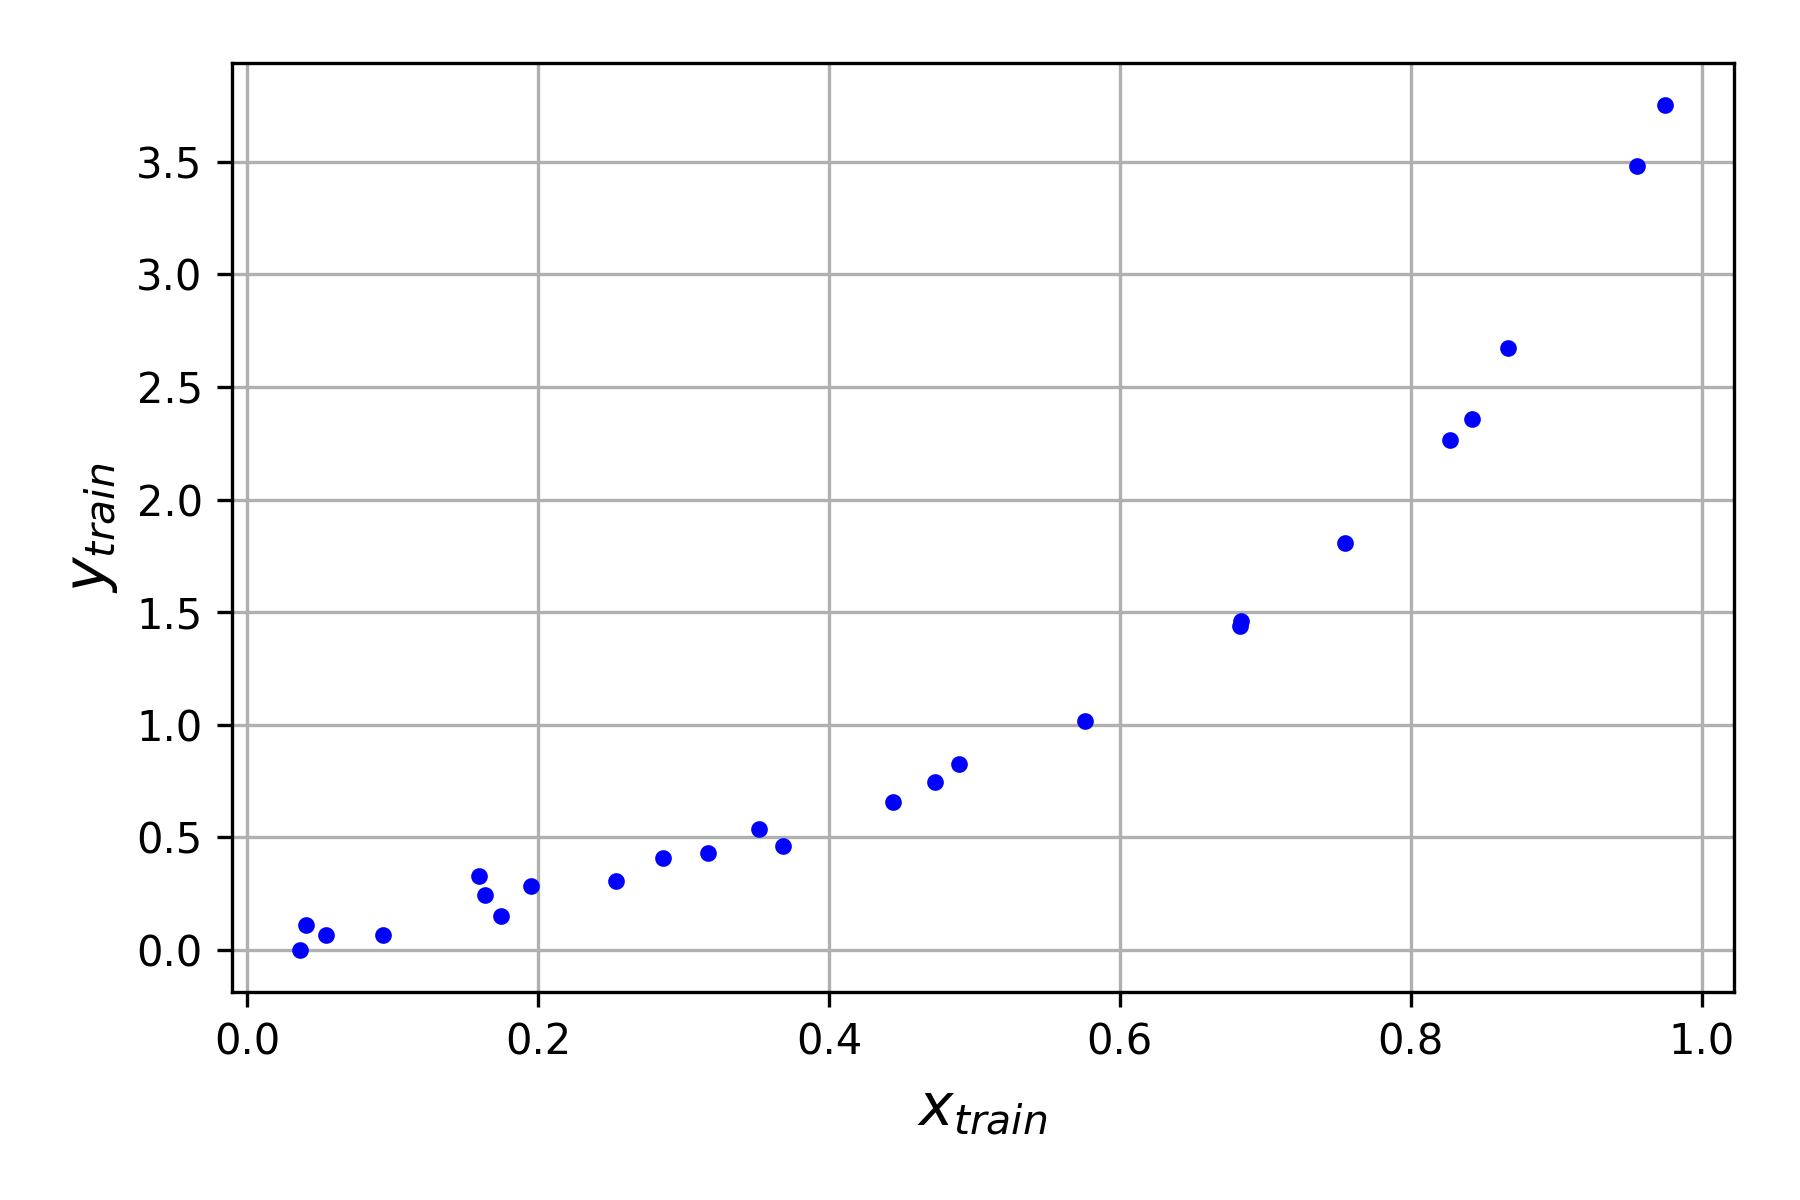
\includegraphics[width=0.7\linewidth]{figures/training_data}
	\caption{Training Data}
\end{figure}
    
    \begin{Verbatim}[commandchars=\\\{\}]
Trainging Dataset size:  (25,)
    \end{Verbatim}
\pagebreak
    \hypertarget{b}{%
\section{(b)}\label{b}}

\hypertarget{i.-5-points-implement-the-following-function-to-make-input-features-for-the-above-linear-regression-model.}{%
\paragraph{i. (5 points) Implement the following function to make input
features for the above linear regression
model.}\label{i.-5-points-implement-the-following-function-to-make-input-features-for-the-above-linear-regression-model.}}

    \begin{tcolorbox}[breakable, size=fbox, boxrule=1pt, pad at break*=1mm,colback=cellbackground, colframe=cellborder]
\prompt{In}{incolor}{5}{\boxspacing}
\begin{Verbatim}[commandchars=\\\{\}]
\PY{k}{def} \PY{n+nf}{get\PYZus{}features}\PY{p}{(}\PY{n}{x}\PY{p}{:} \PY{n}{np}\PY{o}{.}\PY{n}{ndarray}\PY{p}{,} \PY{n}{n}\PY{p}{:} \PY{n+nb}{int}\PY{p}{)} \PY{o}{\PYZhy{}}\PY{o}{\PYZgt{}} \PY{n}{np}\PY{o}{.}\PY{n}{ndarray}\PY{p}{:}
    \PY{l+s+sd}{\PYZdq{}\PYZdq{}\PYZdq{}Creates n\PYZhy{}th degree polynomial features for the given vector x.}
\PY{l+s+sd}{    Example usage:}
\PY{l+s+sd}{    get\PYZus{}features(np.array([1.0, 2.0, 3.0]), 3) outputs}
\PY{l+s+sd}{    np.array([  [ 1., 1., 1.],}
\PY{l+s+sd}{                [ 2., 4., 8.],}
\PY{l+s+sd}{                [ 3., 9., 27.]])}
\PY{l+s+sd}{    Args:}
\PY{l+s+sd}{        x: A numpy array of shape (num\PYZus{}examples, ) or (num\PYZus{}examples, 1).}
\PY{l+s+sd}{        n: The degree of the polynomial features.}
\PY{l+s+sd}{    Returns:}
\PY{l+s+sd}{        A matrix of shape (num\PYZus{}examples, n) where the j\PYZhy{}th column is equal to}
\PY{l+s+sd}{        the vector x raised, elementwise, to the power j.}
\PY{l+s+sd}{    \PYZdq{}\PYZdq{}\PYZdq{}}
    
    \PY{c+c1}{\PYZsh{} create an array of powers }
    \PY{n}{powers} \PY{o}{=} \PY{n}{np}\PY{o}{.}\PY{n}{arange}\PY{p}{(}\PY{l+m+mi}{1}\PY{p}{,} \PY{n}{n}\PY{o}{+}\PY{l+m+mi}{1}\PY{p}{)}

    \PY{c+c1}{\PYZsh{} reshape x to have the shape (num\PYZus{}examples, 1) to be compatible with np.power broadcasing}
    \PY{n}{x} \PY{o}{=} \PY{n}{x}\PY{o}{.}\PY{n}{reshape}\PY{p}{(}\PY{o}{\PYZhy{}}\PY{l+m+mi}{1}\PY{p}{,} \PY{l+m+mi}{1}\PY{p}{)}

    \PY{c+c1}{\PYZsh{} construct the design matrix of shape (num\PYZus{}examples, n)}
    \PY{n}{design\PYZus{}matrix} \PY{o}{=} \PY{n}{np}\PY{o}{.}\PY{n}{power}\PY{p}{(}\PY{n}{x}\PY{p}{,} \PY{n}{powers}\PY{p}{)}

    \PY{c+c1}{\PYZsh{} return the design matrix}
    \PY{k}{return} \PY{n}{design\PYZus{}matrix}
\end{Verbatim}
\end{tcolorbox}

    \hypertarget{ii.-10-points-use-the-above-function-to-complete-the-following-implementation.-hint-you-may-use-the-sklearn.linear_model.linearregression-class.}{%
\pagebreak
\paragraph{\texorpdfstring{ii. (10 points) Use the above function to
complete the following implementation. (Hint: you may use the
\texttt{sklearn.linear\_model.LinearRegression}
class.)}{ii. (10 points) Use the above function to complete the following implementation. (Hint: you may use the sklearn.linear\_model.LinearRegression class.)}} \label{ii.-10-points-use-the-above-function-to-complete-the-following-implementation.-hint-you-may-use-the-sklearn.linear_model.linearregression-class.}}

    \begin{tcolorbox}[breakable, size=fbox, boxrule=1pt, pad at break*=1mm,colback=cellbackground, colframe=cellborder]
\prompt{In}{incolor}{6}{\boxspacing}
\begin{Verbatim}[commandchars=\\\{\}]
\PY{k}{def} \PY{n+nf}{fit\PYZus{}and\PYZus{}evaluate}\PY{p}{(}
    \PY{n}{x\PYZus{}train}\PY{p}{:} \PY{n}{np}\PY{o}{.}\PY{n}{ndarray}\PY{p}{,} \PY{n}{y\PYZus{}train}\PY{p}{:} \PY{n}{np}\PY{o}{.}\PY{n}{ndarray}\PY{p}{,}
    \PY{n}{x\PYZus{}val}\PY{p}{:} \PY{n}{np}\PY{o}{.}\PY{n}{ndarray}\PY{p}{,} \PY{n}{y\PYZus{}val}\PY{p}{:} \PY{n}{np}\PY{o}{.}\PY{n}{ndarray}\PY{p}{,}
    \PY{n}{n}\PY{p}{:} \PY{n+nb}{int}
    \PY{p}{)} \PY{o}{\PYZhy{}}\PY{o}{\PYZgt{}} \PY{n}{Tuple}\PY{p}{[}\PY{n+nb}{float}\PY{p}{,} \PY{n+nb}{float}\PY{p}{]}\PY{p}{:}
    
    \PY{l+s+sd}{\PYZdq{}\PYZdq{}\PYZdq{}Fits an n\PYZhy{}th degree polynomial and outputs train and validation MSE.}
\PY{l+s+sd}{    Fits a linear regression model y = sum\PYZus{}\PYZob{}i=1\PYZcb{}\PYZca{}n w\PYZus{}i x\PYZca{}i to the given train}
\PY{l+s+sd}{    set and outputs the mean\PYZhy{}squared\PYZhy{}error (MSE) on train and validation sets.}
\PY{l+s+sd}{    Args:}
\PY{l+s+sd}{    x\PYZus{}train: Input features for the train set. Has shape (num\PYZus{}train, )}
\PY{l+s+sd}{    y\PYZus{}train: Targets (labels) for the train set. Has shape (num\PYZus{}train, )}
\PY{l+s+sd}{    x\PYZus{}val: Input features for the validation set. Has shape (num\PYZus{}val, )}
\PY{l+s+sd}{    y\PYZus{}val: Targets (labels) for the validation set. Has shape (num\PYZus{}val, )}
\PY{l+s+sd}{    n: The degree of the polynomial fit. See the above equation.}
\PY{l+s+sd}{    Returns:}
\PY{l+s+sd}{    (train\PYZus{}mse, val\PYZus{}mse), tuple of MSE on train and validation sets.}
\PY{l+s+sd}{    \PYZdq{}\PYZdq{}\PYZdq{}}

    \PY{c+c1}{\PYZsh{} Generating polynomial features using the defined function}
    \PY{n}{x\PYZus{}poly\PYZus{}train} \PY{o}{=} \PY{n}{get\PYZus{}features}\PY{p}{(}\PY{n}{x\PYZus{}train}\PY{p}{,} \PY{n}{n}\PY{p}{)}
    \PY{n}{x\PYZus{}poly\PYZus{}val}   \PY{o}{=} \PY{n}{get\PYZus{}features}\PY{p}{(}\PY{n}{x\PYZus{}val}\PY{p}{,} \PY{n}{n}\PY{p}{)}
    
    \PY{c+c1}{\PYZsh{} Fitting a linear regression model to the training set}
    \PY{n}{lin\PYZus{}reg} \PY{o}{=} \PY{n}{LinearRegression}\PY{p}{(}\PY{p}{)}
    \PY{n}{lin\PYZus{}reg}\PY{o}{.}\PY{n}{fit}\PY{p}{(}\PY{n}{x\PYZus{}poly\PYZus{}train}\PY{p}{,} \PY{n}{y\PYZus{}train}\PY{p}{)}

    \PY{c+c1}{\PYZsh{} Generate model predictions for the train set and calculate the MSE.}
    \PY{n}{y\PYZus{}predict\PYZus{}train} \PY{o}{=} \PY{n}{lin\PYZus{}reg}\PY{o}{.}\PY{n}{predict}\PY{p}{(}\PY{n}{x\PYZus{}poly\PYZus{}train}\PY{p}{)}
    \PY{n}{train\PYZus{}mse} \PY{o}{=} \PY{n}{mean\PYZus{}squared\PYZus{}error}\PY{p}{(}\PY{n}{y\PYZus{}train}\PY{p}{,} \PY{n}{y\PYZus{}predict\PYZus{}train}\PY{p}{)}

    \PY{c+c1}{\PYZsh{} Similarly, calculate the MSE on the val set.}
    \PY{n}{y\PYZus{}predict\PYZus{}val} \PY{o}{=} \PY{n}{lin\PYZus{}reg}\PY{o}{.}\PY{n}{predict}\PY{p}{(}\PY{n}{x\PYZus{}poly\PYZus{}val}\PY{p}{)}
    \PY{n}{val\PYZus{}mse} \PY{o}{=} \PY{n}{mean\PYZus{}squared\PYZus{}error}\PY{p}{(}\PY{n}{y\PYZus{}val}\PY{p}{,} \PY{n}{y\PYZus{}predict\PYZus{}val}\PY{p}{)}
    
    \PY{k}{return} \PY{n}{train\PYZus{}mse}\PY{p}{,} \PY{n}{val\PYZus{}mse}
\end{Verbatim}
\end{tcolorbox}

\pagebreak
    \hypertarget{c}{%
\section{(c)}\label{c}}

(5 points) Use the above function to calculate and plot train and
validations MSEs against n = 1, 2, . . . , 10. Include this graph in
your answer sheet. Which n value would you pick for your final model?

    \begin{tcolorbox}[breakable, size=fbox, boxrule=1pt, pad at break*=1mm,colback=cellbackground, colframe=cellborder]
\prompt{In}{incolor}{7}{\boxspacing}
\begin{Verbatim}[commandchars=\\\{\}]
\PY{n}{highest\PYZus{}order} \PY{o}{=} \PY{l+m+mi}{10}
\PY{n}{degrees} \PY{o}{=} \PY{n}{np}\PY{o}{.}\PY{n}{arange}\PY{p}{(}\PY{l+m+mi}{1}\PY{p}{,} \PY{n}{highest\PYZus{}order}\PY{o}{+}\PY{l+m+mi}{1}\PY{p}{)}
\PY{n}{Train\PYZus{}MSE} \PY{o}{=} \PY{n}{np}\PY{o}{.}\PY{n}{zeros}\PY{p}{(}\PY{p}{(}\PY{n}{highest\PYZus{}order}\PY{p}{,}\PY{l+m+mi}{1}\PY{p}{)}\PY{p}{)}
\PY{n}{Val\PYZus{}MSE} \PY{o}{=} \PY{n}{np}\PY{o}{.}\PY{n}{zeros}\PY{p}{(}\PY{p}{(}\PY{n}{highest\PYZus{}order}\PY{p}{,}\PY{l+m+mi}{1}\PY{p}{)}\PY{p}{)}

\PY{k}{for} \PY{n}{i} \PY{o+ow}{in} \PY{n+nb}{range}\PY{p}{(}\PY{l+m+mi}{1}\PY{p}{,} \PY{n}{highest\PYZus{}order} \PY{o}{+}\PY{l+m+mi}{1}\PY{p}{)}\PY{p}{:}
    
    \PY{n}{train\PYZus{}mse}\PY{p}{,} \PY{n}{val\PYZus{}mse} \PY{o}{=} \PY{n}{fit\PYZus{}and\PYZus{}evaluate}\PY{p}{(}
        \PY{n}{dataset}\PY{p}{[}\PY{l+m+mi}{0}\PY{p}{]}\PY{p}{,} \PY{n}{dataset}\PY{p}{[}\PY{l+m+mi}{1}\PY{p}{]}\PY{p}{,} \PY{c+c1}{\PYZsh{} x\PYZus{}train, y\PYZus{}train}
        \PY{n}{dataset}\PY{p}{[}\PY{l+m+mi}{2}\PY{p}{]}\PY{p}{,} \PY{n}{dataset}\PY{p}{[}\PY{l+m+mi}{3}\PY{p}{]}\PY{p}{,} \PY{c+c1}{\PYZsh{} x\PYZus{}val, y\PYZus{}val}
        \PY{n}{i}\PY{p}{)} \PY{c+c1}{\PYZsh{} The degree of the polynomial to fit}

    \PY{n}{Train\PYZus{}MSE}\PY{p}{[}\PY{n}{i}\PY{o}{\PYZhy{}}\PY{l+m+mi}{1}\PY{p}{]} \PY{o}{=} \PY{n}{train\PYZus{}mse}
    \PY{n}{Val\PYZus{}MSE}\PY{p}{[}\PY{n}{i}\PY{o}{\PYZhy{}}\PY{l+m+mi}{1}\PY{p}{]} \PY{o}{=} \PY{n}{val\PYZus{}mse}


\PY{n}{plt}\PY{o}{.}\PY{n}{figure}\PY{p}{(}\PY{n}{figsize}\PY{o}{=}\PY{p}{(}\PY{l+m+mi}{6}\PY{p}{,} \PY{l+m+mi}{4}\PY{p}{)}\PY{p}{)}
\PY{n}{plt}\PY{o}{.}\PY{n}{plot}\PY{p}{(}\PY{n}{degrees}\PY{p}{,} \PY{n}{Train\PYZus{}MSE}\PY{p}{,} \PY{l+s+s2}{\PYZdq{}}\PY{l+s+s2}{r\PYZhy{}\PYZhy{}o}\PY{l+s+s2}{\PYZdq{}}\PY{p}{,} \PY{n}{label}\PY{o}{=}\PY{l+s+s2}{\PYZdq{}}\PY{l+s+s2}{Train MSE}\PY{l+s+s2}{\PYZdq{}}\PY{p}{)}
\PY{n}{plt}\PY{o}{.}\PY{n}{plot}\PY{p}{(}\PY{n}{degrees}\PY{p}{,} \PY{n}{Val\PYZus{}MSE}\PY{p}{,} \PY{l+s+s2}{\PYZdq{}}\PY{l+s+s2}{b\PYZhy{}\PYZhy{}o}\PY{l+s+s2}{\PYZdq{}}\PY{p}{,} \PY{n}{label}\PY{o}{=}\PY{l+s+s2}{\PYZdq{}}\PY{l+s+s2}{Validation MSE}\PY{l+s+s2}{\PYZdq{}}\PY{p}{)}
\PY{n}{plt}\PY{o}{.}\PY{n}{legend}\PY{p}{(}\PY{n}{loc}\PY{o}{=}\PY{l+s+s2}{\PYZdq{}}\PY{l+s+s2}{upper right}\PY{l+s+s2}{\PYZdq{}}\PY{p}{)}
\PY{n}{plt}\PY{o}{.}\PY{n}{xlabel}\PY{p}{(}\PY{l+s+s2}{\PYZdq{}}\PY{l+s+s2}{\PYZdl{}Degree\PYZdl{}}\PY{l+s+s2}{\PYZdq{}}\PY{p}{)}\PY{p}{;} \PY{n}{plt}\PY{o}{.}\PY{n}{xticks}\PY{p}{(}\PY{n}{degrees}\PY{p}{)}
\PY{n}{plt}\PY{o}{.}\PY{n}{ylabel}\PY{p}{(}\PY{l+s+s2}{\PYZdq{}}\PY{l+s+s2}{\PYZdl{}MSE\PYZdl{}}\PY{l+s+s2}{\PYZdq{}}\PY{p}{,} \PY{n}{rotation}\PY{o}{=}\PY{l+m+mi}{0}\PY{p}{)}\PY{p}{;} \PY{n}{plt}\PY{o}{.}\PY{n}{yscale}\PY{p}{(}\PY{l+s+s2}{\PYZdq{}}\PY{l+s+s2}{log}\PY{l+s+s2}{\PYZdq{}}\PY{p}{)}
\PY{n}{plt}\PY{o}{.}\PY{n}{grid}\PY{p}{(}\PY{p}{)}
\PY{n}{save\PYZus{}fig}\PY{p}{(}\PY{l+s+s2}{\PYZdq{}}\PY{l+s+s2}{train\PYZus{}val\PYZus{}mse}\PY{l+s+s2}{\PYZdq{}}\PY{p}{)}
\PY{n}{plt}\PY{o}{.}\PY{n}{show}\PY{p}{(}\PY{p}{)}
\end{Verbatim}
\end{tcolorbox}

\begin{figure}[h]
	\centering
	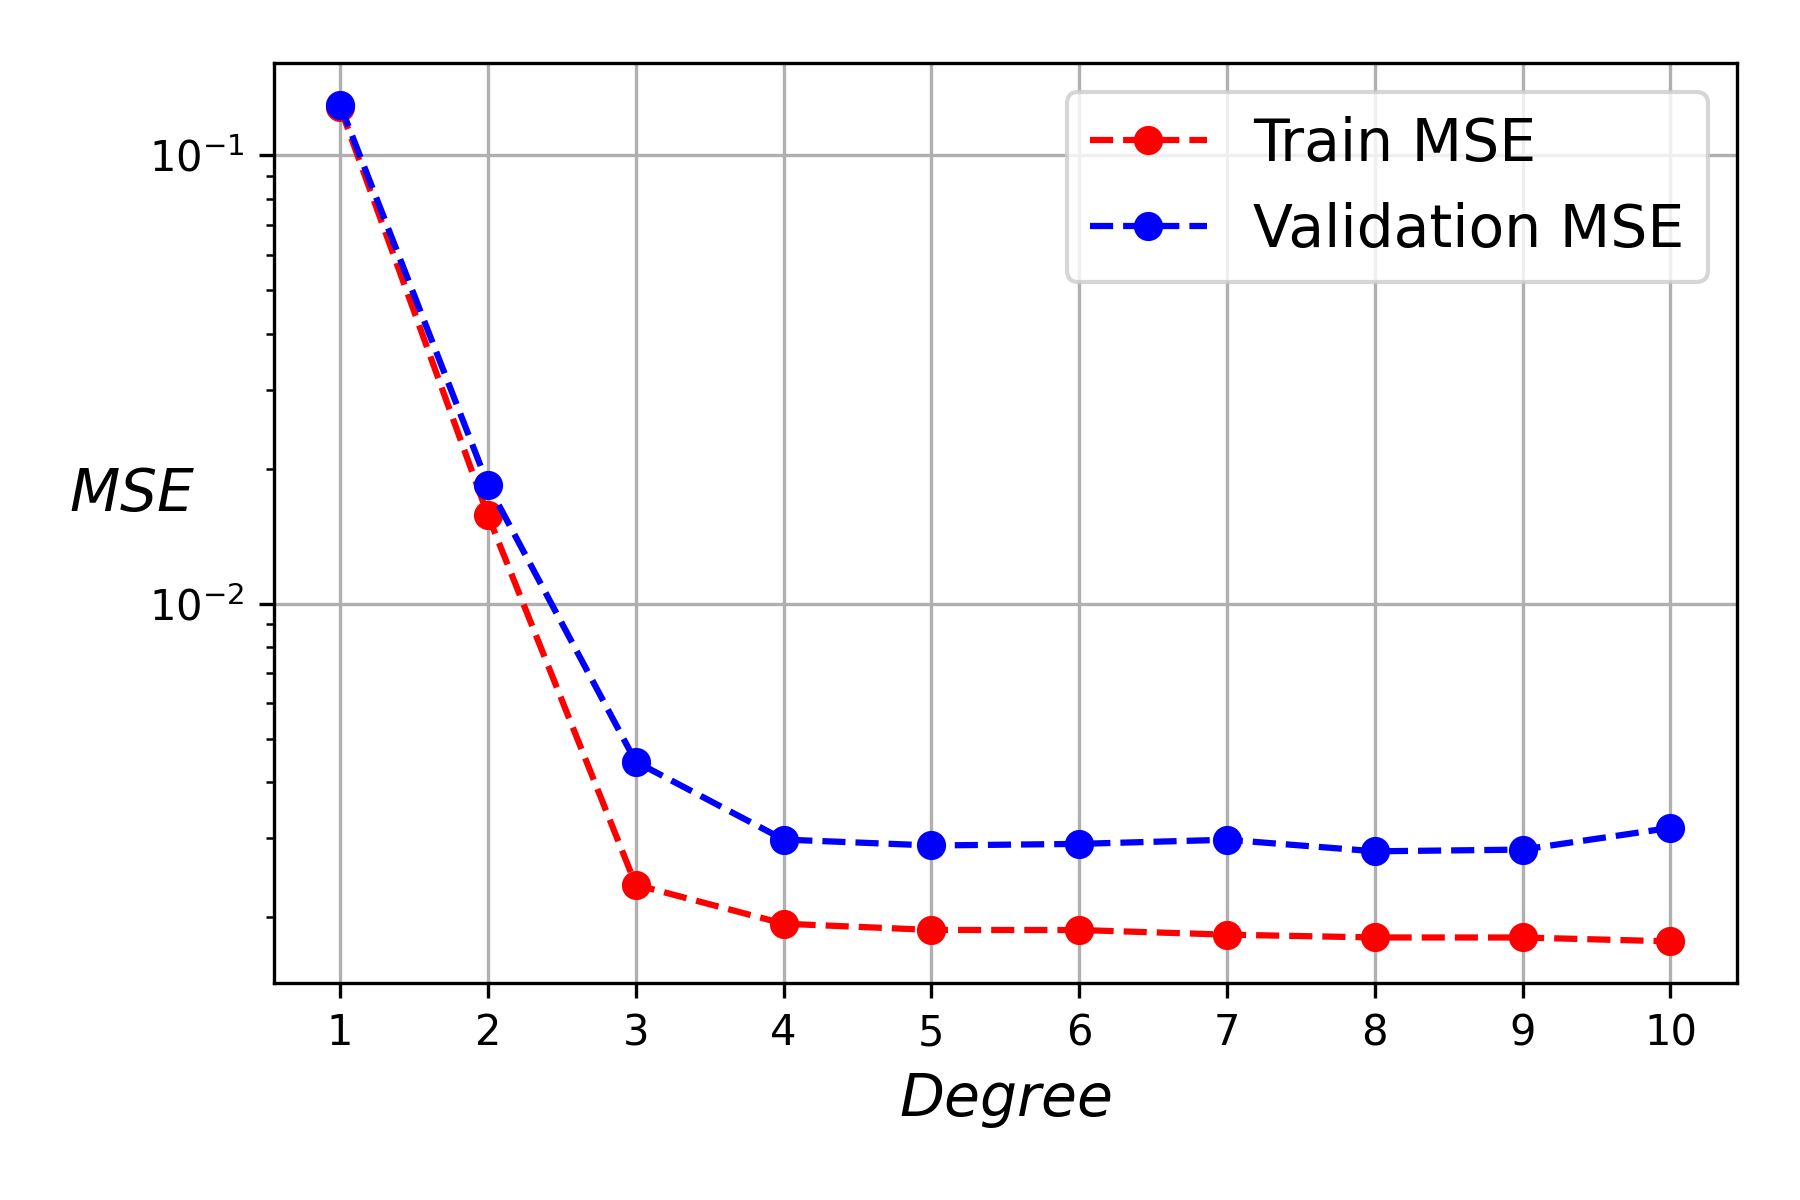
\includegraphics[width=0.7\linewidth]{figures/train_val_mse}
	\caption{Train MSE and Validation MSE}
\end{figure}
   
   \emph{Answer} : According to the learning curves, 4th order polynomial
   fits the data well.
   
    \hypertarget{d}{%
\section{(d)}\label{d}}

(5 points) Use the model selected above to make predictions on the test
set. Include your predictions in a file named
\texttt{\textless{}your-index-number\textgreater{}\_y\_predict\_test.txt}.
For example, \texttt{180000X\_y\_predict\_test.txt}.\\

\emph{Answer} : According to the learning curves, 4th order polynomial
fits the data well.

    \begin{tcolorbox}[breakable, size=fbox, boxrule=1pt, pad at break*=1mm,colback=cellbackground, colframe=cellborder]
\prompt{In}{incolor}{8}{\boxspacing}
\begin{Verbatim}[commandchars=\\\{\}]
\PY{n}{selected\PYZus{}order} \PY{o}{=} \PY{l+m+mi}{4}

\PY{c+c1}{\PYZsh{} Generating polynomial features using the user defined function}
\PY{n}{x\PYZus{}poly\PYZus{}train} \PY{o}{=} \PY{n}{get\PYZus{}features}\PY{p}{(}\PY{n}{dataset}\PY{p}{[}\PY{l+m+mi}{0}\PY{p}{]}\PY{p}{,} \PY{n}{selected\PYZus{}order}\PY{p}{)}

\PY{c+c1}{\PYZsh{} Fitting a linear regression model to the training set}
\PY{n}{lin\PYZus{}reg} \PY{o}{=} \PY{n}{LinearRegression}\PY{p}{(}\PY{p}{)}
\PY{n}{lin\PYZus{}reg}\PY{o}{.}\PY{n}{fit}\PY{p}{(}\PY{n}{x\PYZus{}poly\PYZus{}train}\PY{p}{,} \PY{n}{dataset}\PY{p}{[}\PY{l+m+mi}{1}\PY{p}{]}\PY{p}{)}

\PY{c+c1}{\PYZsh{} predicting on the test data set and save in a file}
\PY{n}{x\PYZus{}poly\PYZus{}test} \PY{o}{=} \PY{n}{get\PYZus{}features}\PY{p}{(}\PY{n}{dataset}\PY{p}{[}\PY{l+m+mi}{4}\PY{p}{]}\PY{p}{,} \PY{n}{selected\PYZus{}order}\PY{p}{)}
\PY{n}{y\PYZus{}predict\PYZus{}test} \PY{o}{=} \PY{n}{lin\PYZus{}reg}\PY{o}{.}\PY{n}{predict}\PY{p}{(}\PY{n}{x\PYZus{}poly\PYZus{}test}\PY{p}{)}
\PY{n}{np}\PY{o}{.}\PY{n}{savetxt}\PY{p}{(}\PY{l+s+s2}{\PYZdq{}}\PY{l+s+s2}{18063J\PYZus{}y\PYZus{}predict\PYZus{}test.txt}\PY{l+s+s2}{\PYZdq{}}\PY{p}{,} \PY{n}{y\PYZus{}predict\PYZus{}test}\PY{p}{)}
\end{Verbatim}
\end{tcolorbox}
\pagebreak
    \hypertarget{visualization}{%
\section{Visualization}\label{visualization}}

    \begin{tcolorbox}[breakable, size=fbox, boxrule=1pt, pad at break*=1mm,colback=cellbackground, colframe=cellborder]
\prompt{In}{incolor}{9}{\boxspacing}
\begin{Verbatim}[commandchars=\\\{\}]
\PY{c+c1}{\PYZsh{} training data}
\PY{n}{plt}\PY{o}{.}\PY{n}{figure}\PY{p}{(}\PY{n}{figsize}\PY{o}{=}\PY{p}{(}\PY{l+m+mi}{6}\PY{p}{,} \PY{l+m+mi}{4}\PY{p}{)}\PY{p}{)}
\PY{n}{plt}\PY{o}{.}\PY{n}{plot}\PY{p}{(}\PY{n}{dataset}\PY{p}{[}\PY{l+m+mi}{0}\PY{p}{]}\PY{p}{,} \PY{n}{dataset}\PY{p}{[}\PY{l+m+mi}{1}\PY{p}{]}\PY{p}{,} \PY{l+s+s2}{\PYZdq{}}\PY{l+s+s2}{g*}\PY{l+s+s2}{\PYZdq{}}\PY{p}{,} \PY{n}{label}\PY{o}{=}\PY{l+s+s2}{\PYZdq{}}\PY{l+s+s2}{Training Data}\PY{l+s+s2}{\PYZdq{}}\PY{p}{)}

\PY{c+c1}{\PYZsh{} data to plot the polynomial}
\PY{n}{data\PYZus{}points} \PY{o}{=} \PY{l+m+mi}{100}
\PY{n}{x} \PY{o}{=} \PY{n}{np}\PY{o}{.}\PY{n}{linspace}\PY{p}{(}\PY{n}{np}\PY{o}{.}\PY{n}{min}\PY{p}{(}\PY{n}{dataset}\PY{p}{[}\PY{l+m+mi}{0}\PY{p}{]}\PY{p}{)}\PY{p}{,} \PY{n}{np}\PY{o}{.}\PY{n}{max}\PY{p}{(}\PY{n}{dataset}\PY{p}{[}\PY{l+m+mi}{0}\PY{p}{]}\PY{p}{)}\PY{p}{,} \PY{n}{data\PYZus{}points}\PY{p}{)}\PY{o}{.}\PY{n}{reshape}\PY{p}{(}\PY{n}{data\PYZus{}points}\PY{p}{,} \PY{l+m+mi}{1}\PY{p}{)}
\PY{n}{x\PYZus{}poly} \PY{o}{=} \PY{n}{get\PYZus{}features}\PY{p}{(}\PY{n}{x}\PY{p}{,} \PY{n}{selected\PYZus{}order}\PY{p}{)}
\PY{n}{y} \PY{o}{=} \PY{n}{lin\PYZus{}reg}\PY{o}{.}\PY{n}{predict}\PY{p}{(}\PY{n}{x\PYZus{}poly}\PY{p}{)}
\PY{n}{plt}\PY{o}{.}\PY{n}{plot}\PY{p}{(}\PY{n}{x}\PY{p}{,} \PY{n}{y}\PY{p}{,} \PY{l+s+s2}{\PYZdq{}}\PY{l+s+s2}{r\PYZhy{}}\PY{l+s+s2}{\PYZdq{}}\PY{p}{,} \PY{n}{linewidth}\PY{o}{=}\PY{l+m+mi}{2}\PY{p}{,} \PY{n}{label}\PY{o}{=}\PY{l+s+s2}{\PYZdq{}}\PY{l+s+s2}{Predictions}\PY{l+s+s2}{\PYZdq{}}\PY{p}{)}

\PY{n}{plt}\PY{o}{.}\PY{n}{legend}\PY{p}{(}\PY{n}{loc}\PY{o}{=}\PY{l+s+s2}{\PYZdq{}}\PY{l+s+s2}{upper left}\PY{l+s+s2}{\PYZdq{}}\PY{p}{)}
\PY{n}{plt}\PY{o}{.}\PY{n}{xlabel}\PY{p}{(}\PY{l+s+s2}{\PYZdq{}}\PY{l+s+s2}{\PYZdl{}X\PYZdl{}}\PY{l+s+s2}{\PYZdq{}}\PY{p}{)}
\PY{n}{plt}\PY{o}{.}\PY{n}{ylabel}\PY{p}{(}\PY{l+s+s2}{\PYZdq{}}\PY{l+s+s2}{\PYZdl{}Y\PYZdl{}}\PY{l+s+s2}{\PYZdq{}}\PY{p}{,} \PY{n}{rotation}\PY{o}{=}\PY{l+m+mi}{0}\PY{p}{)}
\PY{n}{plt}\PY{o}{.}\PY{n}{grid}\PY{p}{(}\PY{p}{)}
\PY{n}{save\PYZus{}fig}\PY{p}{(}\PY{l+s+s2}{\PYZdq{}}\PY{l+s+s2}{predictions}\PY{l+s+s2}{\PYZdq{}}\PY{p}{)}
\PY{n}{plt}\PY{o}{.}\PY{n}{show}\PY{p}{(}\PY{p}{)}
\end{Verbatim}
\end{tcolorbox}

\begin{figure}[h]
	\centering
	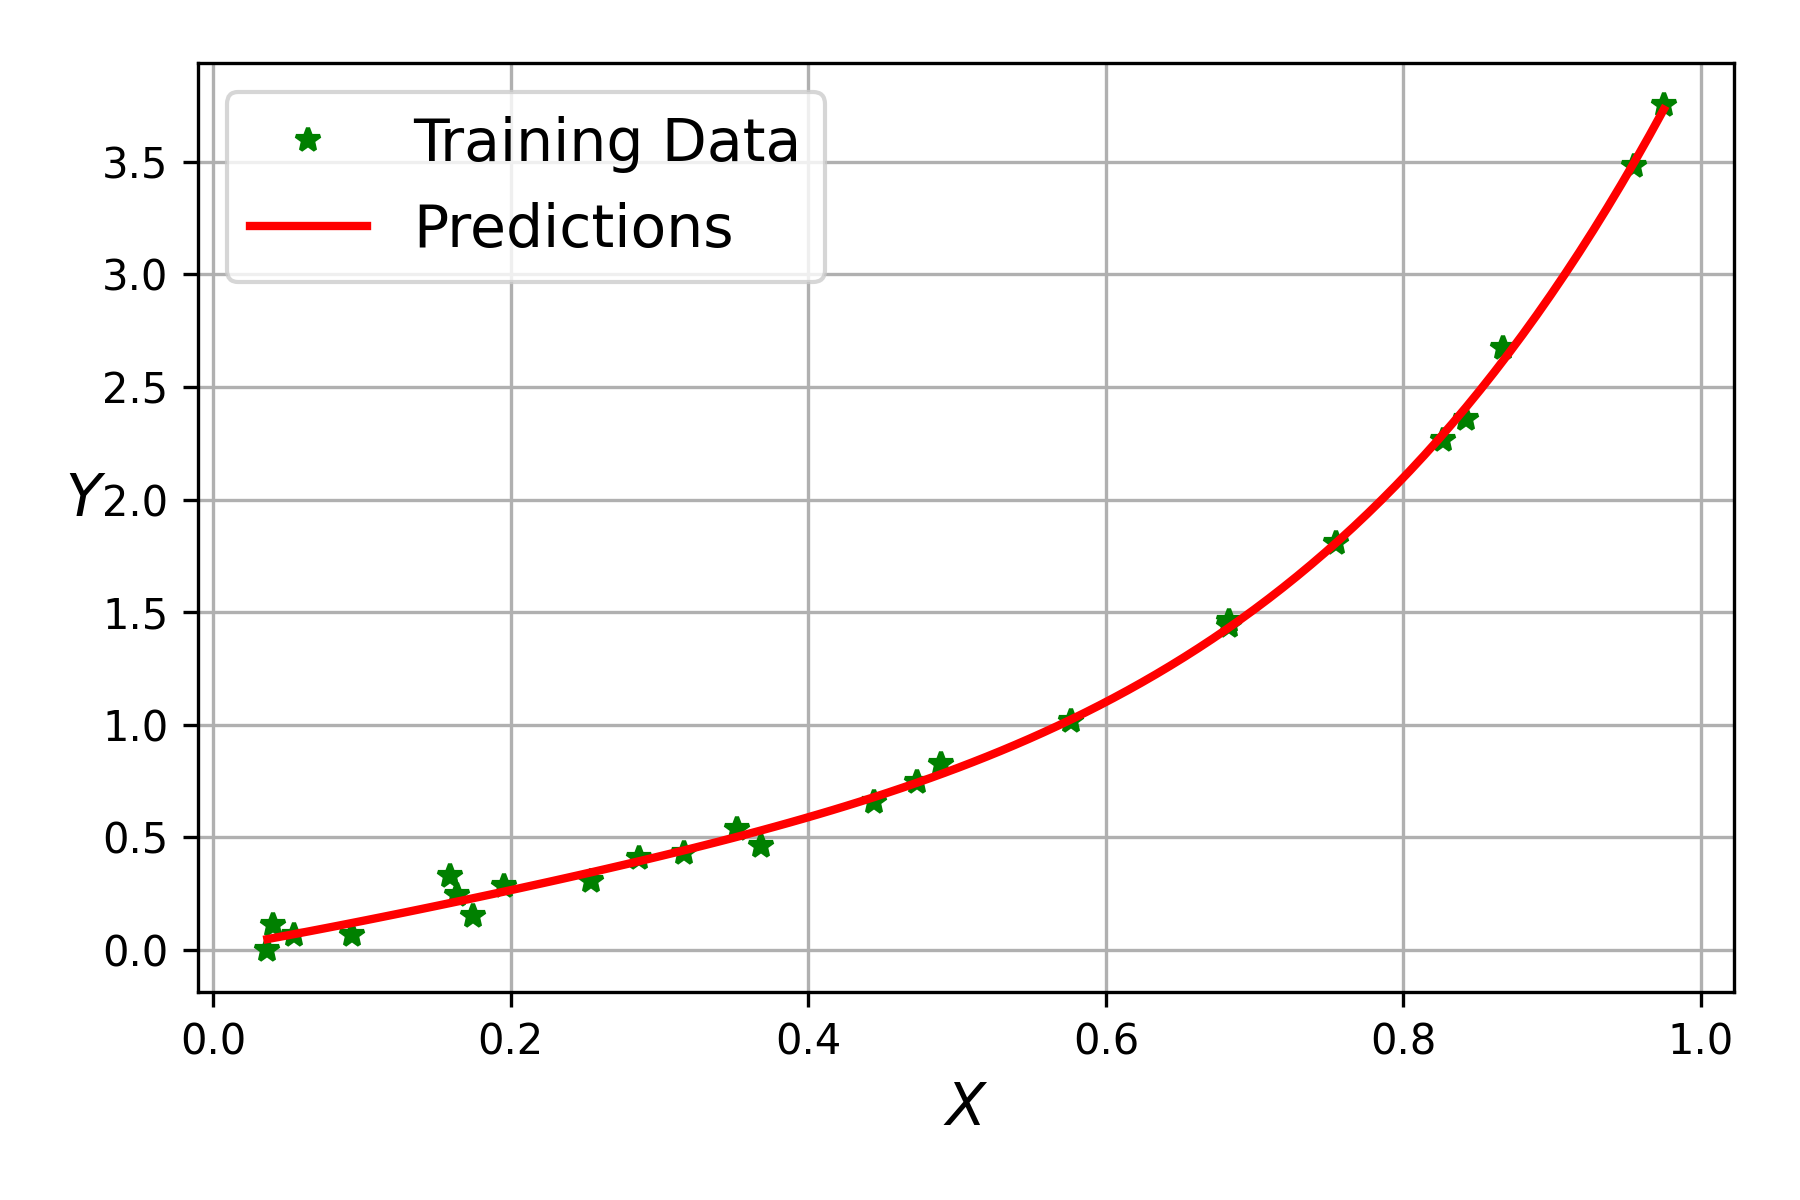
\includegraphics[width=0.7\linewidth]{figures/predictions}
	\caption{Predictions and the Training Data}
\end{figure}
   
\end{document}
